% http://www.ctan.org/tex-archive/macros/latex/contrib/beamer/examples
% http://latex.artikel-namsu.de/english/beamer-examples.html

%\documentclass{beamer}
\documentclass[usenames,dvipsnames]{beamer}
\usepackage{amsmath}
\usepackage{amssymb}
\usepackage{bm}
\usepackage{fancybox, graphicx}
\usepackage{listings}
\usepackage{tikz} % Diagrams
\usepackage{color}
\usepackage{textcomp} % See https://tex.stackexchange.com/questions/145416/how-to-have-straight-single-quotes-in-lstlistings
\usepackage{multicol}
\usepackage{caption}

\lstset{language=bash,upquote=true} % Format listings as appropriate for bash. Inexplicably we get problems if the language is set as part of the \begin{lstlisting} command.

% https://tex.stackexchange.com/questions/36030/how-to-make-a-single-word-look-as-some-code
\definecolor{light-gray}{gray}{0.95}
\newcommand{\code}[1]{\colorbox{light-gray}{\texttt{#1}}}

\newcommand{\mentiurl}[0]{{\url{www.menti.com}}}
\newcommand{\menticode}[0]{{262943}}
\newcommand{\mentiinvitation}[0]{Go to \mentiurl{} (code \menticode{}) and choose one possibility:\\}
\newcommand{\correctanswer}[1]{\textcolor{blue}{{#1} \checkmark}}


\usetheme{boxes}
\usecolortheme{beaver}


\title{How to See Invisible Matter}
\author{Lorne Whiteway \\ lorne.whiteway@star.ucl.ac.uk}
\institute{Astrophysics Group \\ Department of Physics and Astronomy \\ University College London}
\date{21 May 2020}

\subject{IT}

\begin{document}

\frame{\titlepage}


\begin{frame}{Interactive content}
  \begin{block}{}
    You are invited to go to\\
    \begin{center}
    \huge \alert{\mentiurl{}}\\
    \end{center}
    and enter code\\
    \begin{center}
    \huge \menticode{}
    \end{center}
  \end{block}
\end{frame}

\begin{frame}{Goal}
  \begin{block}{}
    We can't see Dark Matter. But can we nevertheless figure out where in the Universe it is located?
  \end{block}
\end{frame}

\begin{frame}{Cosmology}
  \begin{block}{}
    Cosmology is the study of the Universe on the largest scales.
  \end{block}
  \begin{block}{}
    Some parts of cosmology are easy, because we can ignore all the small-scale details \ldots
  \end{block}
\end{frame}

\begin{frame}{Pillars of Cosmology}
  There is strong evidence that:
  \begin{block}{}
    \begin{itemize}
      \item{The Universe is more-or-less the same everywhere and we are not in a `special' location.}
      \item{Einstein's theory (`General Relativity') correctly describes how gravity works.}
      \item{The overall geometry of the Universe is `flat': keep going in a straight line and you won't return home.}
      \item{There was a Big Bang - an initial uniformly dense and hot state - and the Universe has been expanding and cooling ever since.}
    \end{itemize}
  \end{block}
\end{frame}

\begin{frame}{What does the Universe contain?}
    \mentiinvitation{}
    \begin{enumerate}
      \item{Left-over light from the Big Bang, the 'cosmic background radiation', dominates all other forms of energy}
      \item{About 75\% hydrogen, 24\% helium, 1\% everything else}
      \item{5\% gas and stars; the rest we don't really know}
    \end{enumerate}
\end{frame}


\begin{frame}{What does the Universe contain?}
    \begin{enumerate}
      \item{Left-over light from the Big Bang, the 'cosmic background radiation', dominates all other forms of energy}
      \item{About 75\% hydrogen, 24\% helium, 1\% everything else}
      \item{\correctanswer{5\% gas and stars; the rest we don't really know}}
    \end{enumerate}
\end{frame}


\begin{frame}{Contents of the Universe (remember mass = energy!)}
  \begin{block}{}
    \begin{itemize}
      \item{0.01\% light}
      \item{5\% `normal' matter - stars and gas}
      \item{26\% Dark Matter - some form of matter that doesn't interact with light.}
      \item{69\% Dark Energy - ? - mass of empty space?}
    \end{itemize}
  \end{block}
\end{frame}


\begin{frame}{What is Dark Matter?}
  \begin{block}{}
    \begin{itemize}
      \item{We don't know \ldots}
      \item{Range of possible particle masses covers 78 orders of magnitudes \ldots}
      \item{No interaction with light, so dark and invisible.}
      \item{Particle physicists have been searching for years - no luck \ldots}
      \item{But like all forms of mass/energy, it interacts via gravity.}
    \end{itemize}
  \end{block}
\end{frame}


\begin{frame}{Simulations}
  \begin{block}{}
    \begin{itemize}
      \item{We can run computer simulations in which we follow the trajectories of dark matter particles under the influence of gravity.}
	\item{I ran a simulation - using software `PKDGRAV3' - following one billion dark matter `lumps'  from the beginning of time to today.}
    \end{itemize}
  \end{block}
\end{frame}

\begin{frame}{Simulation result - note log scale}
    \centering
    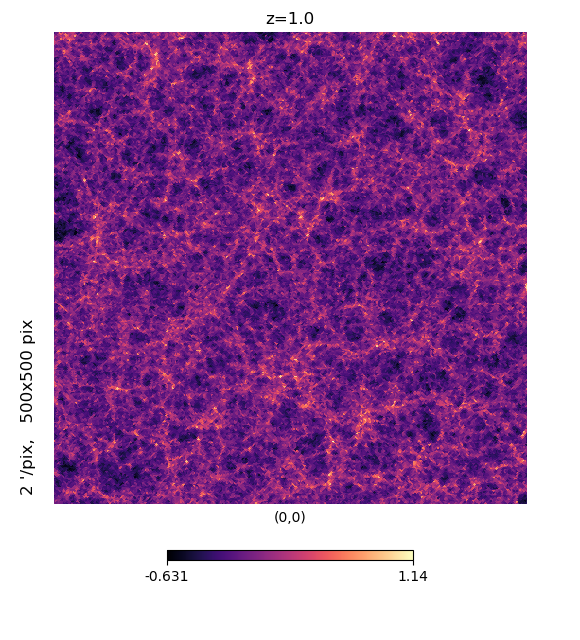
\includegraphics[height=8cm]{simulation_z_1.png}
\end{frame}
  

\begin{frame}{Simulation result}
  \begin{columns}
    \column{0.56\linewidth}
    \begin{itemize}
      \item{The dark matter clusters into large `halos' - the densest areas in the picture.}
      \item{Hydrogen gas is pulled into the densest halos, where it forms galaxies.}
	\item{Also there are `filaments' of dark matter joining the haloes, so we get a `cosmic web'.}
    \end{itemize}
    \column{0.4\linewidth}
    \centering
    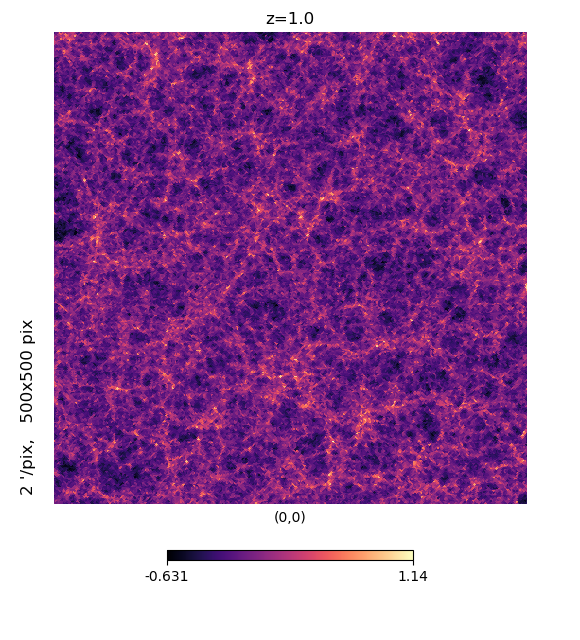
\includegraphics[height=5cm]{simulation_z_1.png}
  \end{columns}
\end{frame}


\begin{frame}{Why are there no dark matter galaxies and stars?}
  \begin{block}{}
    \mentiinvitation{}
    \begin{enumerate}
      \item{Dark matter particles move too fast - near the speed of light.}
      \item{Dark matter can't cool down by emitting light.}
      \item{Gravity acts only weakly on dark matter.}
    \end{enumerate}
  \end{block}
\end{frame}


\begin{frame}{Why are there no dark matter galaxies and stars?}
  \begin{block}{}
    \begin{enumerate}
      \item{Dark matter particles move too fast - near the speed of light.}
      \item{\correctanswer{Dark matter can't cool down by emitting light.}}
      \item{Gravity acts only weakly on dark matter.}
    \end{enumerate}
  \end{block}
\end{frame}

\begin{frame}{Goal}
  \begin{block}{}
    \begin{itemize}
      \item{We want to map the distribution of dark matter on cosmological scales.}
      \item{We can't see dark matter \ldots}
      \item{\ldots but we can infer its location from its gravitational impact on light from distant galaxies.}
      \item{Our main tool is `weak lensing' (WL)}
    \end{itemize}
  \end{block}
\end{frame}


\begin{frame}{Weak lensing}
  \begin{block}{}
    \begin{itemize}
      \item{The gravity of dark matter bends space and hence bends the trajectory of light from distant galaxies.}
      \item{This has three effects on the appearance of distant galaxies.}
    \end{itemize}
  \end{block}
\end{frame}


\begin{frame}{The effects of bending light}
  \begin{columns}
    \column{0.56\linewidth}
    \begin{itemize}
      \item{Light gets deflected by the dark matter\ldots}
      \item{\ldots which moves the image of the galaxy on the sky \ldots}
	\item{\ldots and distorts it (makes it flatter i.e. ellipses become more eccentric) \ldots}
	\item{\ldots and can magnify it.}
	\item{Of these, it's the \textbf{distortion} that we choose to investigate.}
    \end{itemize}
    \column{0.4\linewidth}
    \centering
    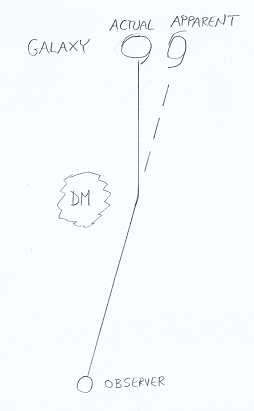
\includegraphics[height=6cm]{diagram_1.png}
  \end{columns}
\end{frame}


\begin{frame}{Which lensing effect is the practical one to study?}
  \begin{block}{}
    \mentiinvitation{}
    \begin{enumerate}
      \item{The change in location}
      \item{The change in shape (eccentricity)}
      \item{The change in brightness}
    \end{enumerate}
  \end{block}
\end{frame}

\begin{frame}{Which lensing effect is the practical one to study?}
  \begin{block}{}
    \begin{enumerate}
      \item{The change in location}
      \item{\correctanswer{The change in shape (eccentricity)}}
      \item{The change in brightness}
    \end{enumerate}
  \end{block}
\end{frame}


\begin{frame}{That's crazy!}
  \begin{columns}
    \column{0.56\linewidth}
    \begin{itemize}
      \item{The effect on shapes must be minuscule!}
      \item{It is - it's just at the edge of detectability.}
      \item{But with shapes we at least know the \textbf{distribution} of shapes before the effect of lensing.}
      \item{For example, the `angle $\Theta$ of major axis` should be uniformly distributed.}
    \end{itemize}
    \column{0.4\linewidth}
    \centering
    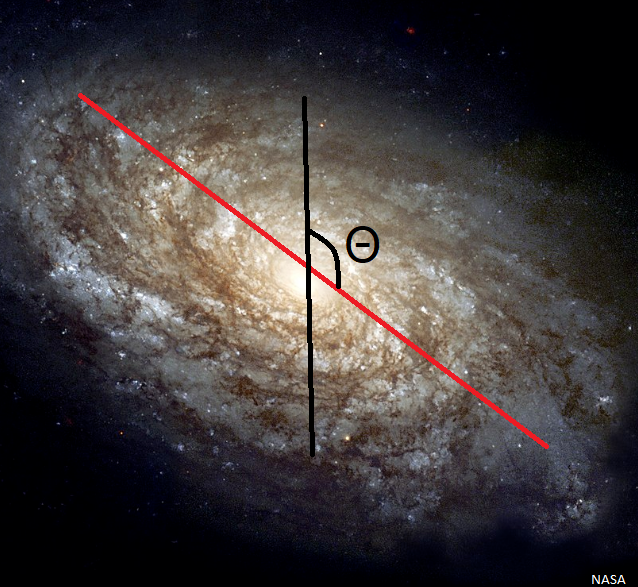
\includegraphics[height=4.5cm]{diagram_2.png}
  \end{columns}
\end{frame}

\begin{frame}{Weak lensing}
    \centering
    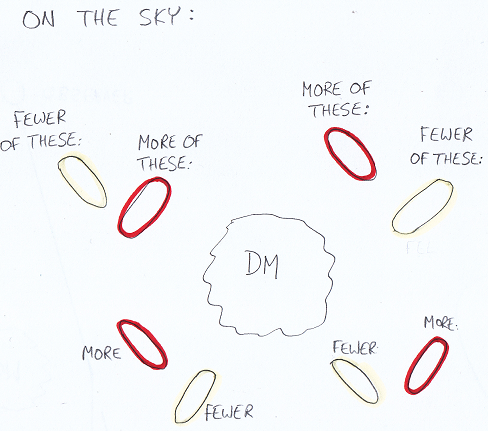
\includegraphics[height=8cm]{diagram_3.png}
\end{frame}


\begin{frame}{Weak lensing}
  \begin{block}{}
    So if we see such a quadrupole bias in the shapes, we can infer that there is dark matter in the centre of the picture.
  \end{block}
\end{frame}


\begin{frame}{Strong lensing versus Weak lensing}
    \centering
    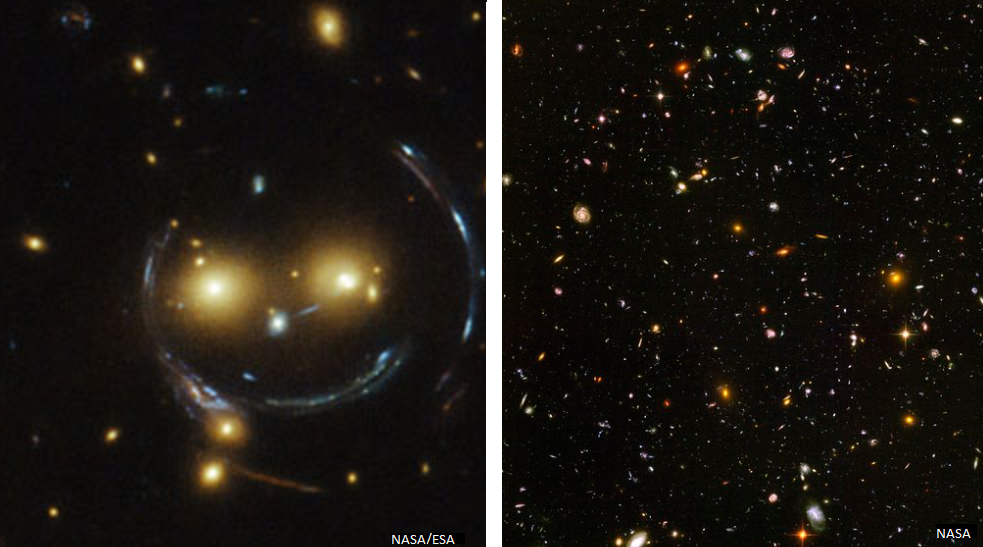
\includegraphics[height=6cm]{diagram_4.png}
\end{frame}

\begin{frame}{Low signal-to-noise ratio}
  \begin{block}{}
    \begin{itemize}
      \item{The effect on the shapes of galaxies is about 1\% of the intrinsic scatter in the shapes themselves.}
      \item{In other words, the \textbf{signal} is 1\% of the \textbf{noise}.}
      \item{So the SNR (signal-to-noise ratio) is about 0.01  - that's very low!}
      \item{Only way to overcome this is with \textit{lots} of data.}
    \end{itemize}
  \end{block}
\end{frame}

\begin{frame}{SNR = 0.01 - how many data points needed?}
  \begin{block}{}
    \mentiinvitation{}
    \begin{enumerate}
      \item{100}
      \item{1,000}
      \item{10,000}
    \end{enumerate}
  \end{block}
\end{frame}

\begin{frame}{SNR = 0.01 - how many data points needed?}
  \begin{block}{}
    \begin{enumerate}
      \item{100}
      \item{1,000}
      \item{\correctanswer{10,000}}
    \end{enumerate}
  \end{block}
\end{frame}

\begin{frame}{How to get so much data?}
  \begin{block}{}
    \begin{itemize}
      \item{Fortunately there are \textbf{lots} of galaxies! We just have to photograph them all \ldots}
      \item{There have been several \textit{weak lensing surveys} taking long exposure photographs of large areas of the sky.}
      \item{For example, the DES project covered one-eighth of the sky; each part of this area was photographed for about 75 minutes.}
      \item{It currently has a catalogue of the shapes of 100,000,000 galaxies.}
    \end{itemize}
  \end{block}
\end{frame}

\begin{frame}{It's all statistics}
  \begin{block}{}
    \begin{itemize}
      \item{Analysing so much low-SNR data requires careful statistical treatment.}
      \item{We usually work within the framework of \textit{Bayesian} statistics.}
    \end{itemize}
  \end{block}
\end{frame}

\begin{frame}{What does Bayes's Theorem say?}
  \begin{block}{}
    \mentiinvitation{}
    \begin{enumerate}
      \item{Posterior proportional to Likelihood times Prior}
      \item{Likelihood proportional to Posterior times Prior}
      \item{Prior proportional to Likelihood times Posterior}
    \end{enumerate}
  \end{block}
\end{frame}

\begin{frame}{What does Bayes's Theorem say?}
  \begin{block}{}
    \begin{enumerate}
      \item{\correctanswer{Posterior proportional to Likelihood times Prior}}
      \item{Likelihood proportional to Posterior times Prior}
      \item{Prior proportional to Likelihood times Posterior}
    \end{enumerate}
  \end{block}
\end{frame}

\begin{frame}{What does Bayes's Theorem say?}
  \begin{block}{}
  The \textit{posterior} probability of a parameter depends both on:
    \begin{itemize}
      \item{the \textit{likelihood} of seeing the observed data (given the parameter), and}
      \item{the \textit{prior} probability of the parameter (before the experiment started).}
    \end{itemize}
  \end{block}
\end{frame}


\begin{frame}{Bayes example}
  \begin{columns}
    \column{0.56\linewidth}
    \begin{itemize}
      \item{Strangely-shaped trees? Or old glass?}
      \item{Both explanations fit the picture equally well (same \textit{likelihood})!}
      \item{But old glass is more common than strange trees (has more \textit{prior} probability).}
      \item{So we conclude `old glass' has more \textit{posterior} probability.}
    \end{itemize}
    \column{0.4\linewidth}
    \centering
    % The image file BDP1F0.jpg is from alamy.com. On 20 May 2020 I purchased image rights. See AlamyInvoice.pdf for details.
    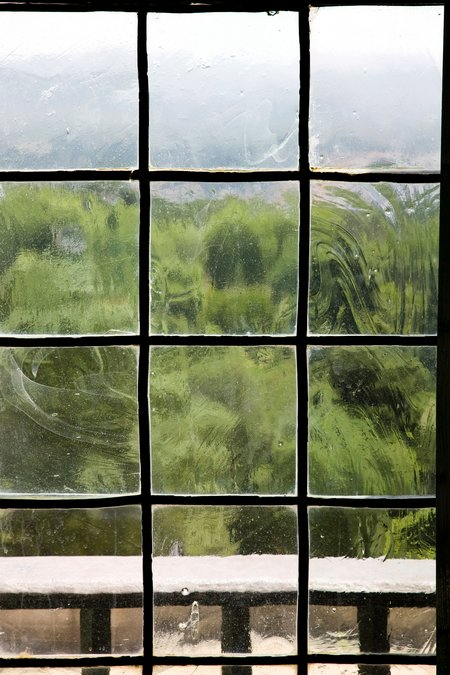
\includegraphics[height=6cm]{BDP1F0.jpg}
  \end{columns}
\end{frame}


\begin{frame}{Bayes and Weak Lensing}
  \begin{columns}
    \column{0.56\linewidth}
    In weak lensing we seek an answer - i.e. a map of the dark matter - that both:
      \begin{itemize}
        \item{is consistent with the observed galaxy shapes, and}
        \item{has a high prior probability (i.e. is physically plausible).}
      \end{itemize}
    If we don't insist on the latter condition then we end up just fitting noise.
    \column{0.4\linewidth}
    \centering
    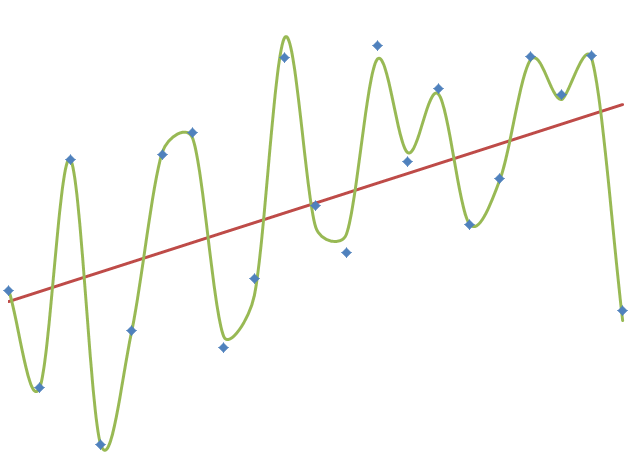
\includegraphics[height=3cm]{diagram_5.png}
  \end{columns}
\end{frame}

\begin{frame}{GLIMPSE algorithm}
  \begin{columns}
    \column{0.56\linewidth}
    \begin{block}{}
      \begin{itemize}
        \item{Currently I'm using the GLIMPSE algorithm (Lanusse et al. arXiv:1603.01599)}
        \item{This algorithm assigns a high prior probability to patterns in the dark matter density that are combinations of a small number of \textit{wavelets}.}
        \item{A wavelet is a cosine wave that has been smoothly truncated at each end.}
      \end{itemize}
    \end{block}
    \column{0.4\linewidth}
    \centering
    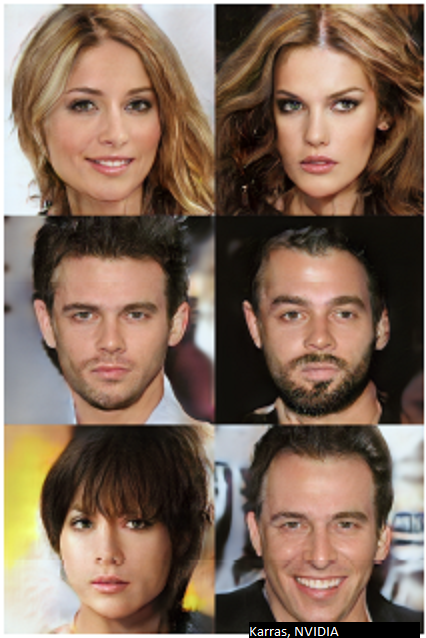
\includegraphics[height=4cm]{diagram_6.png}
  \end{columns}
\end{frame}





 
\end{document}
